\documentclass[tikz,border=12pt]{standalone}
\usepackage[T1]{fontenc}
\begin{document}
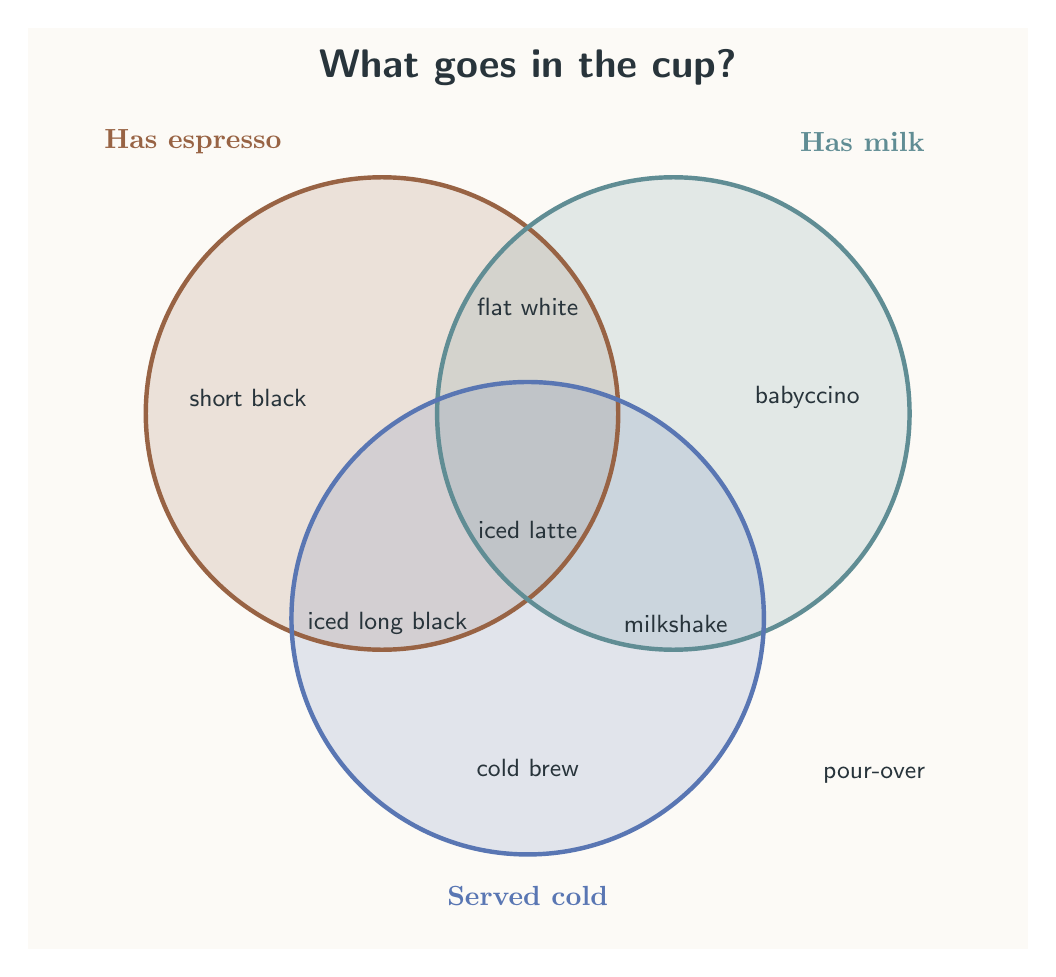
\begin{tikzpicture}[font=\sffamily, line join=round]
  \definecolor{espresso}{HTML}{986344}
  \definecolor{milk}{HTML}{608D94}
  \definecolor{cold}{HTML}{5976B3}
  \definecolor{ink}{HTML}{28343B}
  \definecolor{paper}{HTML}{FCFAF6}
  \path[use as bounding box] (-6.35,-5.65) rectangle (6.35,6.05);
  \fill[paper] (-6.35,-5.65) rectangle (6.35,6.05);
  \node[font=\sffamily\bfseries\Large, text=ink] at (0,5.55) {What goes in the cup?};
  % Three translucent sets: the overlap is visible without obscuring the words.
  \fill[espresso,opacity=.16] (-1.85,1.15) circle (3);
  \fill[milk,opacity=.16] (1.85,1.15) circle (3);
  \fill[cold,opacity=.16] (0,-1.45) circle (3);
  \draw[espresso,line width=1.6pt] (-1.85,1.15) circle (3);
  \draw[milk,line width=1.6pt] (1.85,1.15) circle (3);
  \draw[cold,line width=1.6pt] (0,-1.45) circle (3);
  % Set names sit just outside the corresponding outlines.
  \node[font=\bfseries, text=espresso] at (-4.25,4.60) {Has espresso};
  \node[font=\bfseries, text=milk] at (4.25,4.60) {Has milk};
  \node[font=\bfseries, text=cold] at (0,-4.97) {Served cold};
  % Drinks in all seven occupied regions, plus the drink in no set.
  \tikzset{drink/.style={text=ink,font=\sffamily\small,align=center,inner sep=2pt}}
  \node[drink] at (-3.55,1.35) {short black};
  \node[drink] at (3.55,1.35) {babyccino};
  \node[drink] at (0,2.50) {flat white};
  \node[drink] at (-1.78,-1.52) {iced long black};
  \node[drink] at (1.88,-1.52) {milkshake};
  \node[drink] at (0,-0.33) {iced latte};
  \node[drink] at (0,-3.35) {cold brew};
  \node[drink] at (4.40,-3.45) {pour-over};
\end{tikzpicture}
\end{document}
